\section{Theory}
\subsection{Modulus of Elasticity}

Young's Modulus or Modulus of Elasticity of a material is defined as the ratio of longitudinal stress and the corresponding longitudinal strain.

\begin{equation}
    Y = \frac{FL_0}{A\Delta L}
\end{equation}

Here, $F/A$ is the force applied per unit area, and $\Delta L/L$ is the extension cause by the applied force with respect to the initial length $L$.

Usually when a sample material is stretched in one direction, it tends to get thinner in the other direction. Poisson's ratio is the measure of this tendency and is defined as the ratio of the strain in the direction of applied load to the strain in the transverse direction. A perfectly in-compressible material has Poisson’s ratio $\sigma = 0.5$.

\begin{figure}[H]
    \centering
    \label{fig:3}
    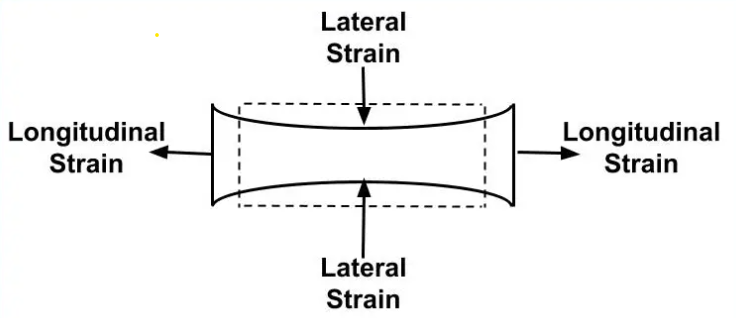
\includegraphics[width=0.8\columnwidth]{images/f2.png}
    \caption{Schematic diagram of the deformation of a material under longitudinal stress}
\end{figure}

\subsection{Experimental Principle}
Cornu proposed a method to measure the deformation of a solid under load using the interference phenomenon of light. According to his method, a glass plate is kept on top of a glass beam and load is applied on both sides of the glass beam. Therefore, the glass beam will be deformed due to strain in the longitudinal direction (x-axis), and since Poisson's ration $\sigma \ne 0$, it will also be deformed in the transverse direction (y-axis).Thus the beam deforms into the shape of horse saddle forming a thin film of air between them. When the film is illuminated by monochromatic light, interference occurs between the light reflected from the bottom of the glass plate and the top of the beam as shown in Fig. 1.

Let $x$ and $y$ be the coordinates along longitudinal and transverse direction centering around $O$. Also, let $R_x$ and $R_y$ be the radius of curvature of the glass beam in longitudinal and transverse directions respectively. In order to obtain the shape of the interference fringes, consider that the thickness of air film between the glass plate and the beam to be $t(x,y)$ at a point (x,y) in the XY-plane. 

\begin{figure}[H]
    \centering
    \label{fig:1}
    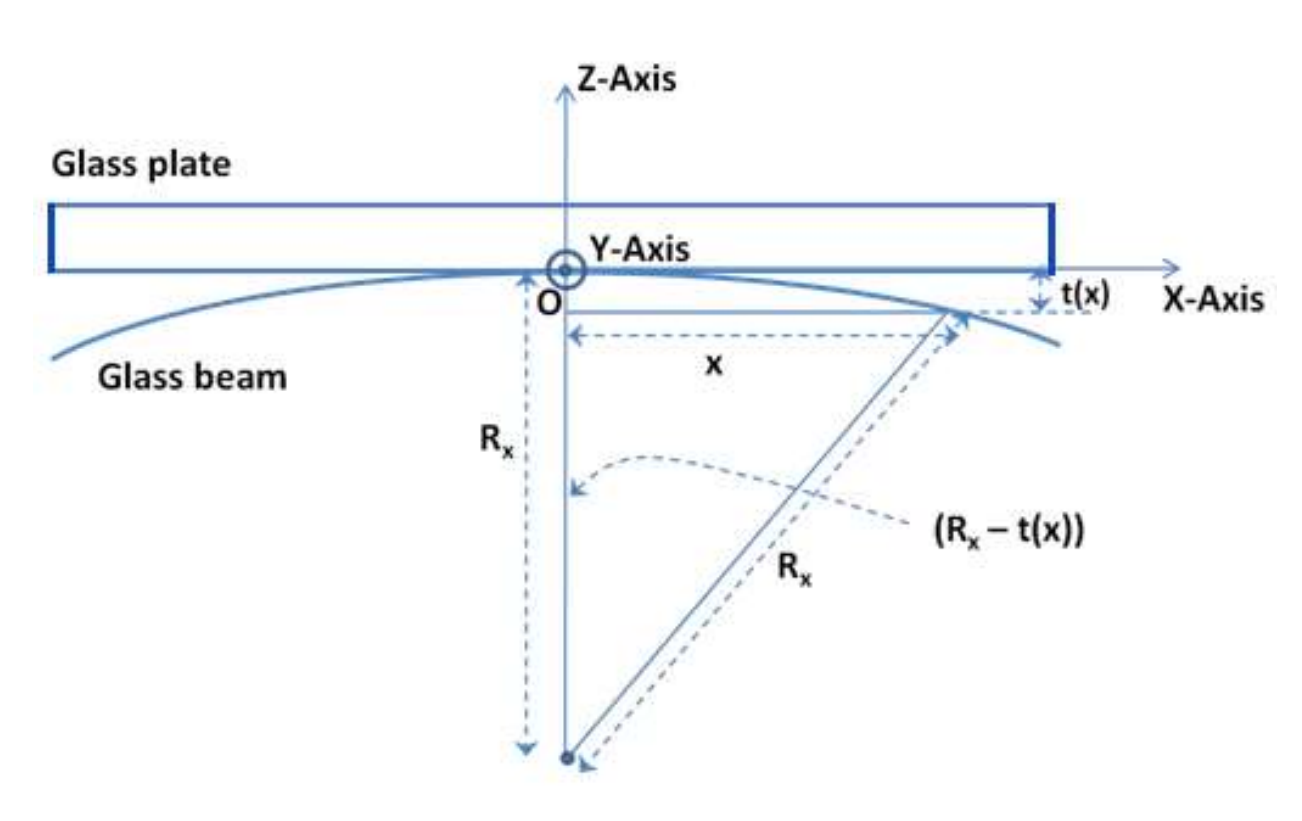
\includegraphics[width=1\columnwidth]{images/f1.png}
    \caption{Schematic drawing of the geometry to obtain the fringes}
\end{figure}

Firstly, consider the $x$ dependence of $t(x,y)$ i.e. $t(x)$. As evident in Fig 1, we can obtain $t(x)$ as:
\begin{equation}
    (R_x - t(x))^2 = R_x^2 - x^2
\end{equation}

Assuming $t(x)$ to be very small, we get
\begin{equation}
    t(x) = \frac{x^2}{2R_x}
\end{equation}

Similarly, $t(y)$ can be obtained from
\begin{equation}
    t(y) = -\frac{y^2}{2R_y}
\end{equation}
Here, there appears a negative sign because the glass beam bends upwards along the transverse direction (y-axis). Thus, $t(x, y)$ can be expressed as
\begin{equation}
    t(x, y)=\frac{x^2}{2R_x}-\frac{y^2}{2R_y}
\end{equation}

The fringe shapes are determined by the locus of all points with identical path difference, in the case, constant thickness, i.e. $t(x,y)$ is constant.
\begin{equation}
    \frac{x^2}{2R_x}-\frac{y^2}{2R_y} = a^2
\end{equation}
which represents the equation of a hyperbola, where $a$ is a constant. So, the fringes will be hyperbolic in nature (Fig. 2).

\begin{figure}[H]
    \centering
    \label{fig:2}
    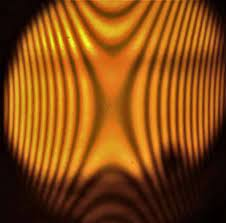
\includegraphics[width=1\columnwidth]{images/f3.jpg}
    \caption{Hyperbolic fringes observed through the travelling microscope}
\end{figure}

The light waves passing through glass plate will be divided into two parts --- one from the reflection from the bottom of the glass plate-air interface and the second one from the top of air film-glass
beam interface (which would under go a phase change of $\pi$ due to reflection at the air film-glass beam interface and would traverse the width of the air film twice). These two components would interfere and produce the fringe pattern.
Therefore, the optical phase difference between these two waves (for almost normal incidence) is
given by,

\begin{equation}
    \Delta \phi = \frac{2\pi}{\lambda}(2\mu t(x, y)) + \pi
\end{equation}

Where $\mu$ is the refractive index of the air film and $\lambda$ is the wavelength of light. Let's assume $\mu$ = 1 for air. If the $N^{th}$ dark fringe along the x-axis is at a distance $x_N$ from the origin, then the interfering waves are out of phase by,

\begin{align}
    & \Delta \phi = (2N + 1)\pi \\
     \Rightarrow & 2t_N(x) = \frac{x_N^2}{R_x}=N\lambda \\
    \text{and, } & 2t_{N+s}(x) = \frac{x_{N+s}^2}{R_x}=(N+s)\lambda
\end{align}

where $x_{N+s}$ is the $(N+s)^{th}$ dark fringe along x-axis. Subtracting eqn. (9) from (10) we get,

\begin{equation}
    R_x =  \frac{x_{N+s}^2 - x_N^2}{s\lambda} = \frac{\rho_x(s)}{s\lambda}
\end{equation}

where we define $\rho_x(s) = x_{N+s}^2 - x_N^2$ for convenience.

Since it is difficult to find the origin, we measure the diameter (D) of the fringe, which is the distance between the N-th dark fringe on the right and left sides correspondingly. Hence $D_{N_x} = 2x_N$.

Once the radius of curvature $R_x$ is obtained, we relate it to the internal bending moment of the glass slab, given by

\begin{equation}
    G_x = \frac{Ybd^3}{12}\frac{1}{R_x} = \frac{Ybd^3}{12}\frac{s\lambda}{\rho_x(s)}
\end{equation}

where $b$ and $d$ and $Y$ are the thickness, depth and Young's Modulus of the glass beam respectively. This internal bending moment will be balanced by the external bending moment applied by the loads hanging from the beam.\\
If $l$ is the distance between the knife-edge and the suspension point of the load (of mass $m$ each), hanging on both sides, then we can write,

\begin{equation}
    (mg)l = \frac{Ybd^3}{12}\frac{s\lambda}{\rho_x(s)}
\end{equation}

If we carry out the measurements for two different loads, we can obtain this expression to calculate the  \textbf{Young's modulus} of the glass beam as,

\begin{equation}
    (m_1 - m_2)gl = \frac{Ybd^3}{12}s\lambda\left(\frac{1}{\rho_{x}^2}-\frac{1}{\rho_{x}^3}\right)
\end{equation}

To Calculate Poisson's Ratio, we need the ratio of radius of curvature of the fringes in the longitudinal direction to that in the transverse direction. Similar to the process of finding $R_x$ in eqn. (11), we can obtain $R_y$ using,

\begin{equation}
    R_y =  \frac{y_{N+s}^2 - y_N^2}{s\lambda} = \frac{\rho_y(s)}{s\lambda}
\end{equation}

Thus, \textbf{Poisson's ratio} can be calculated by,

\begin{equation}
    \sigma =  \frac{R_x}{R_y} = \frac{\rho_x(s)}{\rho_y(s)}
\end{equation}
